\section{Approach}
This section is divided into two subsections. The first describes the methodology of our approach
to the project, while the second describes the schedule we plan to follow.

\subsection{Methodology}
Our project will be available for free use. It will feature a simple, intuitive user interface experience,
and a more sophisticated, database-driven backend to gather, sort, and filter the appropriate data 
when responding to user interaction.

The frontend will feature:
\begin{enumerate}
\item A way to manually create schedules by entering course numbers, and display the resulting schedule in a 
pleasing graphical form. This will largely consist of a text box and some drop-down menus for selecting 
sections within each course.
\item A way to view more information about the courses offered, both in the form of a course list and in
more detailed information about each course on-demand. This will take the form of a search box above a long 
list of courses, sorted by course number, each of which links to a smaller page containing more details about
the course.
\item A way to automatically generate schedules based on a list of constraints provided by the user. This will
consist of a sequence of text and check boxes where the user may select various options for their schedules,
as well as various priorities for classes that they would like to take. These parameters are then fed into a 
modified interval scheduling algorithm, which will attempt to produce a reasonably optimal schedule given the
user's desires.
\end{enumerate}

The backend will be written largely in Python, using the Flask web framework. The database containing class
and user information will be accessed using the mySQL bindings. This will allow the website to be quickly
iterated upon, as making changes is easy given the brevity and clarity of code written using this method.
In order to populate our database, we will write a simple web crawler which will pull the data from Carnegie
Mellon's publicly available Schedule of Classes page. We believe that doing so is the best way to provide
users with up-to-date, complete information.

\subsection{Project Schedule}
We plan to have the data gathered, as well as the basics of our functionality done,
by three weeks into the project. From there, we will spend our time refining the user
experience, as well as improving the quality of our automatic scheduling algorithms. 
If there is enough time, we will extend the application to allow for more sophisticated
constraints to be requested. If we finish exceptionally early, we may also extend the
site to recommend courses based on past course history and future plans.
By the third week of November, we will have finished all features being worked on and
moved to fully polishing and debugging the existing site, as well as prepare our
final report and presentation.
Figure 1 below shows a more detailed view of our proposed schedule.
\begin{figure}[h!]
  \centering
  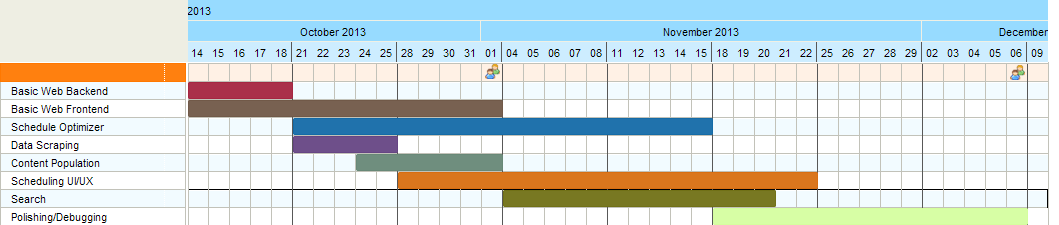
\includegraphics[width=\textwidth]{gantt.png}
  \caption{Gantt chart of the project schedule}
\end{figure}